\documentclass{article}[12pt]

\usepackage{mathptmx}
\usepackage{amssymb}
\usepackage{graphicx}

\begin{document}


%%%%%%%%%%%%%%%%%%%%%%%%%%%%%%%%
\section{Product of $4$ consecutive integers}

Show that the product of $4$ consecutive integers $P(k) = k.(k+1).(k+2).(k+3)$
is a multiple of $4!$
\bigskip

Solution.

Two methods are possible here, one is purely arithmetic and the other one is geometric.

\begin{enumerate}
\item The result directly follows from the following facts:

In $4$ consecutive integers, at least two are even, one of both even is a multiple of $4$.
In $3$ consecutive integers, at least one in a multiple of $3$.
\item
The geometric construction is tricky and comes from a representation of the product $P(k)$ as a rectangle whose sides are the product of the two extreme factors 
$k.(k+3)$ by the two internal factors $(k+1)(k+2)$.

$k.(k+3) = k^2 + 3k$ and $(k+1)(k+2) = k^2 + 3k +2$, thus, $P(k)$ is almost a square (a square minus 1)
if the last column is put as the last rows as shown in the figure.

We can even go further since the elementary pattern is a triangular number which is divisible by $3$:

The side of this square
$k^2+3k+1$ is odd. 

$\Delta_{3k-1} = \frac{3k.(3k-1)}{2}$
\end{enumerate}


\begin{figure}[h]
\begin{center}
        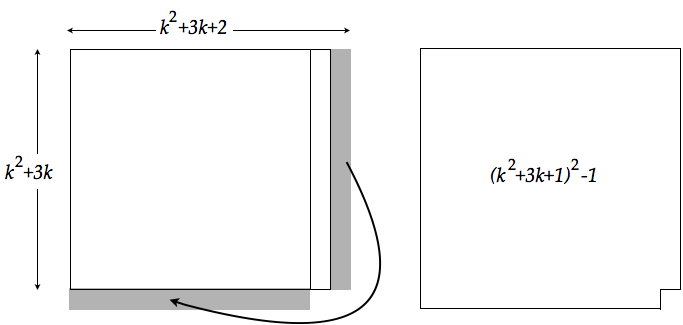
\includegraphics[scale=0.5]{FiguresArithmetic/Product4consecutivePhase1} 
        \caption{The rectangle $k.(k+3)$ by $(k+1)(k+2)$. Moving the last column in grey (left) 
        in place of an extra row gives almost a perfect square (right).}
\end{center}
\end{figure}
\begin{figure}[h]
\begin{center}
        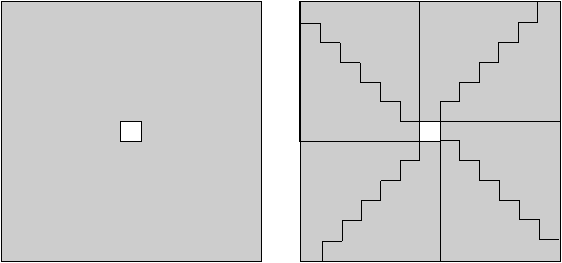
\includegraphics[scale=0.5]{FiguresArithmetic/Product4consecutivePhase2} 
        \caption{Dividing the internal area of a odd square into $8$ equal pieces.}
\end{center}
\end{figure}



%%%%%%%%%%%%%%%%%%%%%%%%%%%%%%%%
\section{Exercise}

Let consider a suite of triangles that contain smaller size equilateral $(1,1,1)$ triangles. 
The objective here is to enumerate all equilateral triangles for each index of the progression
(see Fig.~\ref{fig:countingTriangles}).
The goal is to compute the elements of the progression.
\begin{figure}[h]
\begin{center}
        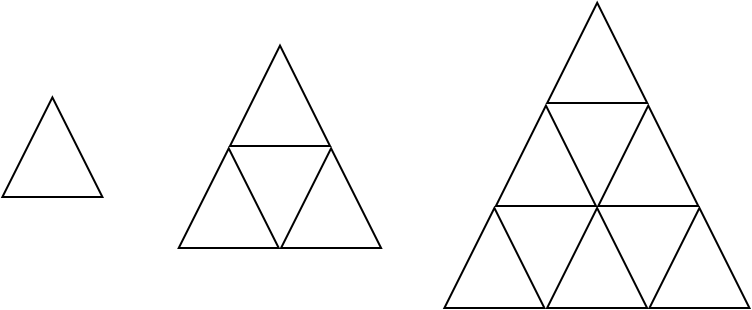
\includegraphics[scale=0.4]{FiguresArithmetic/CountingTriangles} 
        \caption{The first three triangles of the progression.}
        \label{fig:countingTriangles}
\end{center}
\end{figure}

The first terms of the progression are $1$ and $5$ ($4$ small triangles and a large one).

Compute this number for the third term.

Draw the fourth term and compute its number.

Solution.

Let denote the k-th term by $N_k$.

$N_1=1$, $N_2=4$ (one large and 4 small triangles) and $N_3=13$ (1 large, 3 medium and 9 small ones).
\\

Hint: Let do an enumeration is as follows:
\begin{enumerate}
\item
$N_3 = 10$
\item 
$N_4 = 27$.

Fig.~\ref{fig:countingTriangles2} and Fig.~\ref{fig:countingTriangles3}
provides a clear enumeration (from small to large triangles).
\end{enumerate}

Notice that the number of the smallest triangles at rank $k$ corresponds to the sum of odds
which is equal to $k^2$ (according to the result proved in chapter Summation).
\begin{figure}[h]
\begin{center}
        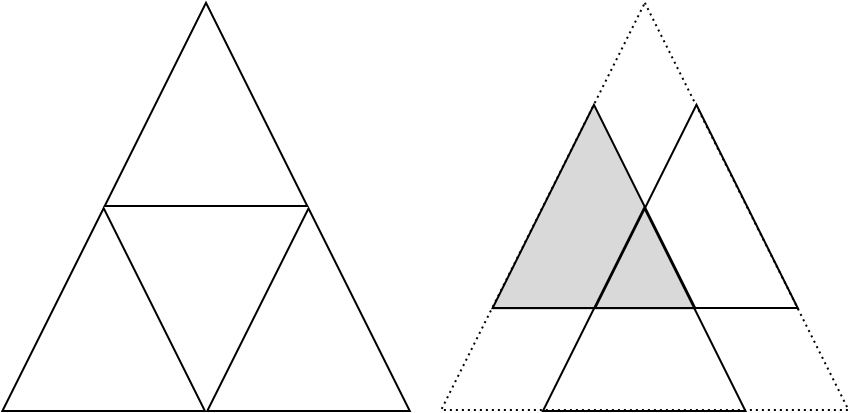
\includegraphics[scale=0.3]{FiguresArithmetic/CountingTriangles2} 
        \caption{7 triangles at level 2 triangles (4 + 3).}
        \label{fig:countingTriangles2}
\end{center}
\end{figure}
\begin{figure}[h]
\begin{center}
        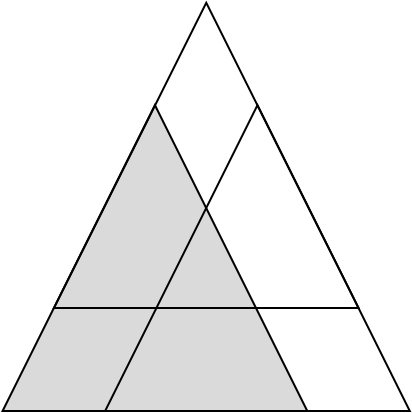
\includegraphics[scale=0.3]{FiguresArithmetic/CountingTriangles3} 
        \caption{3 triangles at level 3.}
        \label{fig:countingTriangles3}
\end{center}
\end{figure}
\bigskip

The solution is:

$N_k = \frac{k.(k+2).(2k+1)}{8}$ for $k$ even

$N_k = \frac{k.(k+2).(2k+1)-1}{8}$ for $k$ odd
\bigskip

The expressions can be derived by the following trick:
Make the difference between two consecutive numbers and again and again, then, the pattern is obvious
(alternance of $2$ and $1$, ...). See Fig.~\ref{fig:countingTrianglesproof}.
\begin{figure}[h]
\begin{center}
        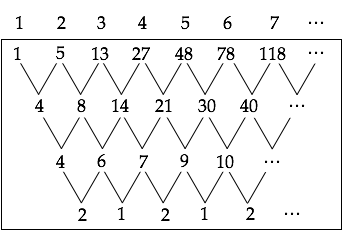
\includegraphics[scale=0.5]{FiguresArithmetic/CountingTrianglesProof} 
        \caption{Computing the differences of consecutive $N_k$.}
        \label{fig:countingTrianglesProof}
\end{center}
\end{figure}
\bigskip

Still, the solution is not obvious.

Consider the last two lines.
The problem is determining a closed expression for the sequence is rather easy:

$2 \rightarrow 6$

$4 \rightarrow 9$

$6 \rightarrow 12$

$8 \rightarrow 15$

$f_1(k) = 3.(\frac{k}{2}+1)$

$f_2(k) = f_1(k) - 2$, thus $f_2(k) = \frac{3}{2}(k+1)+1$


%%%%%%%%%%%%%%%%%%%%%%%%%%%%%%%%
\section{Exercise}


Euler version of the proof of infinite number of primes.



%%%%%%%%%%%%%%%%%%%%%%%%%%%%%%%%
\section{Sum of finite geometric progression}

Chapter 6

Extend the geometrical proof for computing the sum of a finite geometric progression ($u_{n+1} = b.u_{n-1}$
and $u_0=1$). 

Solution: use Thales from the reserve side...


%%%%%%%%%%%%%%%%%%%%%%%%%%%%%%%%
\section{Link of perfect number and triangular numbers}

Show that the perfect number $PN_\alpha$ is equal to the $2^\alpha-1$ triangular number.


%%%%%%%%%%%%%%%%%%%%%%%%%%%%%%%%
\section{A special type of permutation: the Monge's shuffle}

A card trick: the Shuffle of Monge.
\bigskip

We are given 2n cards, which are divided evenly into two decks. 
The shuffle corresponds to put them such that the cards in the final deck come alternatively from left to right as depicted 
in Fig~\ref{fig:suffleMonge}.
The order $(1,2,3,4,5,6,7,8)$ becomes $(5,1,6,2,7,3,8,4)$.
\begin{figure}[h]
\begin{center}
        \includegraphics[scale=0.5]{FiguresArithmetic/suffleMonge} 
        \caption{Shuffle for $8$ cards ($n=4$).}
        \label{fig:suffleMonge}
\end{center}
\end{figure}


Let consider a prime $p$ $53$ and an integer $n$ such that $2n+1=p$.
Here $n=26$, $2n=52$ is a usual deck of Poker cards. 

We apply this shuffle several times.

Show that the number of steps of Monge shuffle to come back to the initial deck divides $p-1$. 



%%%%%%%%%%%%%%%%%%%%%%%%%%%%%%%%
\section{Exercise}

Let consider the sum of the $n$ first integers $\Delta_n$.

Show the following expression:
for any positive integer $n$,
\[ \Delta_{n}^2 \ = \ n^3 + \Delta_{n-1}^2 \]

The solution is easy by decomposing $\Delta_{n} = n + \Delta_{n-1}$
and then, developing the square $\Delta_{n}^2 = n^2 + 2.\Delta_{n-1} + \Delta_{n-1}^2$


%%%%%%%%%%%%%%%%%%%%%%%%%%%%%%%%
\section{Exercise}

Prove that 
\[ \Delta_{n} + \Delta_{n-1} \ = \ n^2  \]

The solution is straightforward by any method
(arithmetic manipulations, Fubini double counting principle, geometrical, recurrences, etc.).

we can ask for several proofs, the goal is then to master the big variety of proofs...
\bigskip

Another related expression is to ask for a "similar" expression for:
\[ \Theta_{n} + \Theta_{n-1} \ = \ ?  \]

where $\Theta_n$ is the sum of the $n$ first $\Delta_n$.

The goal here is to guess a mathematical property, and then, to prove it.

$\Theta_{n} + \Theta_{n-1} $ is equal to the sum of the first $n$ squares, which is equal to $\Delta_n^2$.


%%%%%%%%%%%%%%%%%%%%%%%%%%%%%%%%
\section{Pascal triangle}

A deep look at the Pascal triangle.
\bigskip

Draw the first rows of the Pascal triangle.

Observation: determine regularities on rows, columns, diagonals, etc.. 

Prove the following properties

\begin{enumerate}
\item The sum of the element in a row is a power of $2$.
\item 
The elements of the first column are all equal to $1$.
\item  The elements of the second column are the successive integers
\item The elements of the third column are the triangular numbers (sum of first integers)
\item The elements of the fourth column are the tetrahedral numbers, and so on.
\end{enumerate}

%Solution.
%\begin{figure}[h]
%\begin{center}
%        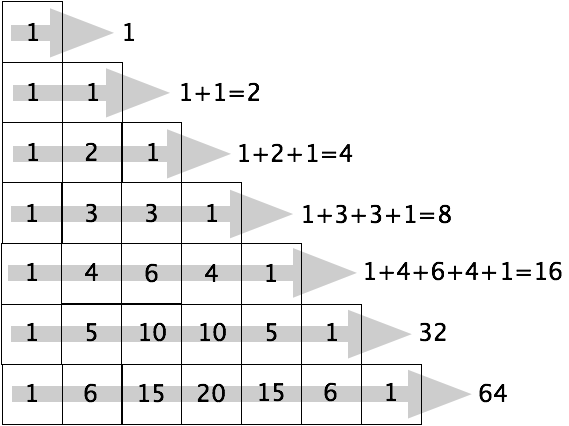
\includegraphics[scale=0.3]{coeffBinomiauxHorizontal} \hspace{1cm}
%         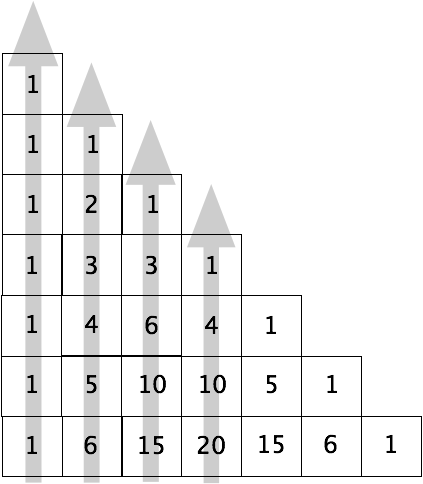
\includegraphics[scale=0.3]{coeffBinomiauxVertical}
%        \caption{Looking at the Pascal's triangle by rows and by columns.}
%\end{center}
%\end{figure}


%%%%%%%%%%%%%%%%%%%%%%%%%%%%%%%%
\section{Binomial coefficients.}


Draw the Pascal's triangle modulo a prime (take for instance $5$).
and explain the geometrical patterns (occurence of the sub-triangle of size $5$ and sub-triangle with $0$.
%\begin{figure}[h]
%\begin{center}
%        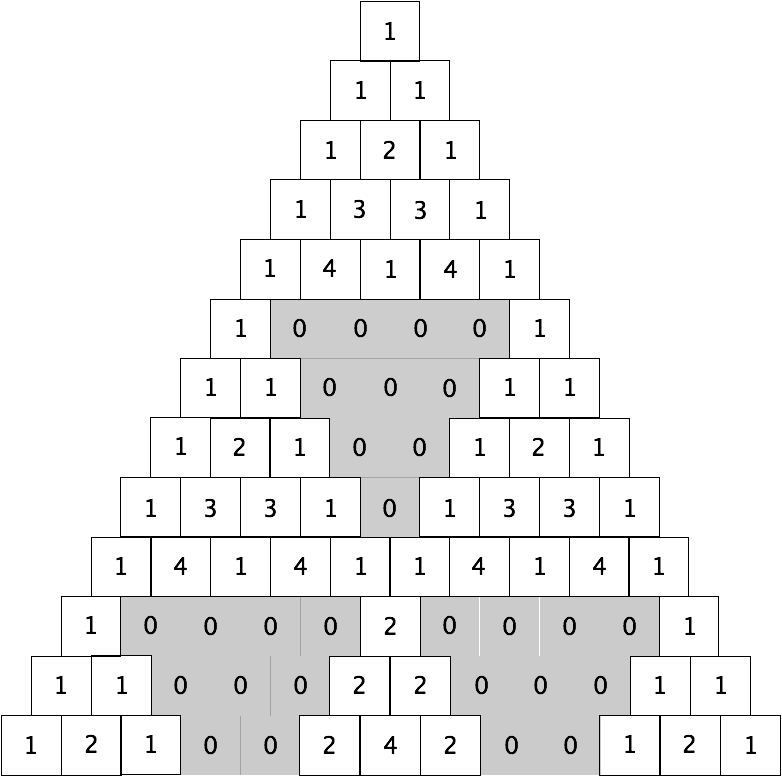
\includegraphics[scale=0.4]{PascalTrianglePrimes}
%        \caption{Regular patterns modulo $5$.}
%\end{center}
%\end{figure}


%%%%%%%%%%%%%%%%%%%%%%%%%%%%%%%%
\section{The Horner-Estrin scheme for polynomial evaluation}

Notice that the analysis leads asymptotically to the same complexity as the classical Horner's scheme but in a different way.
\bigskip

Let consider a polynomial of degree $d$:
\[
P(x) \ \ = \ \ a_0 \ + \ a_1 x \ + \ a_2 x^2 \ + \cdots + \ a_{d-1} x^{d-1} \ + \ a_d x^d
\]

Below is an example for $d=7$.

We rewrite $P(x)$ as:
\[
P(x) \ \ = \ \ a_0 \ + \ a_1 x \ + \ x^2 \ ( a_2  \ + a_3 x \ ) \ + 
\ x^4 \ ( \ a_4 \ + \ a_5 x \ + \ x^2 \ ( a_6  \ + a_7 x \ ) \ )
\]

%\noindent General degree $d$:
%
%$P(x) \ \ = \ \ a_0 \ + \ x \cdot (a_1 \ + \ x \cdot (a_2  \ +  \cdots
%+ x \cdot (a_{d-2} \ + \ x \cdot (a_{d-1} \ + \ a_d x)) \cdots ))$  

We introduce 

$C_i^{(0)} = a_i + x a_{i+1}$ 

$C_i^{(n)} = C_i^{(n-1)} + x^{2n} C_{i+2^n}^{(n-1)}$ 
\bigskip

Write $P(d)$ using the $C_i$ (consider $d$ is a power of $2$ to simplify).

How many additions and multiplications are required?
\bigskip

Solution:
\[
P(x) \ \ = \ \ C_{0}^{(0)} \ + \ x^2 \ C_2^{(0)} \ + 
\ x^4 \ ( \ C_4^{(0)} \ + \ x^2 \ C_6^{(0} \ )
\ = \ C_0^{(1)} \ + \ x^4 \ C_4^{(1)} 
\]

\begin{itemize}
\item
For $d=7$, we have $2$ multiplications for computing $x^2$ and $x^4$
\item
Then, 4 multiplications for the products $a_7 x$,  $a_5 x$, $a_3 x$ and $a_1 x$

followed by 4 additions
\item
2 multiplications for the $x^2 C_2^{(0)}$ and  $x^2 C_6^{(0)}$

followed by 2 additions
\item
Finally, 1 multiplication for computing $x^4 C_4^{(1)}$

followed by 1 addition
\end{itemize}

Total of $2 + 7$ multiplications and $7$ additions.

Generalization: 
$d + log_2(d)$ multiplications and $d$ additions.
\bigskip

This has to be compared to the Horner's scheme: $d$ multiplications and $d$ additions.


%%%%%%%%%%%%%%%%%%%%%%%%%%%%%%%%
\section{Fast multiplication of polynomials}


\subsection{Case study for degree 1}

Let consider $P(x) = a_1 + a_2 x $ and $P'(x) = a'_1 + a'_2 x $

$(P \times P')(x) = (a_1.a'_1) + (a_1.a'_2 + a_2.a'_1) x + (a_2.a'_2) x^2$

The coefficients of this new polynomial require $4$ multiplications and $1$ addition, 
namely $a_1.a'_1$, $a_1.a'_2$, $a_2.a'_1$ and $a_2.a'_2$.
\bigskip

Show how to reduce the number of multiplications using the Karatsuba's trick 
introduced in Exercise~\ref{} that is, 
to use the following arithmetic identity $ad+bc = ac + bd + (b-a)(c-d)$.

\subsection{1 star - Extension}

The goal now is to extend the previous analysis to polynomial of higher degrees.
Let consider that the degree is a power of $2$.
\bigskip

Solution:
Let detail what happens for polynomials of degree $2$:

Let consider $P(x) = a_1 + a_2 x + a_3 x^2$ and $P'(x) = a'_1 + a'_2 x + a'_3 x^2$

$(P \times P')(x) = (a_1.a'_1) + (a_1.a'_2 + a_2.a'_1) x + (a_1.a'_3 + a_2.a'_2 + a_3.a'_1) x^2 + (a_2.a'_3 + a_3.a'_2) x^3 +  (a_3.a'_3) x^4$
\bigskip

Now, write $P(x) = A_1 + A_2 x^2$ 

where $A_1 = a_1 + a_2 x$ and $A_2 = a_3$ and similarly for $P'$

$(P \times P')(x) = (A_1.A'_1) + (A_1.A'_2 + A_2.A'_1) x^2 + (A_2.A'_2) x^4$ 

and apply the same method as before using again the Karatsuba's trick on the $A_i$ and $A'_i$.



%%%%%%%%%%%%%%%%%%%%%%%%%%%%%%%%
\section{Tournament}

Chater 13.

let consider a Directed Acyclic Graph $G$.
Show that every Tournament is hamiltonian.

Definition of Tournament.




\end{document}


